% !TeX root = 00_Vorlage.tex
% !TeX spellcheck = de_DE

\chapter{Aufbau und Methoden}
\label{sec:aufbau}
In diesem Kapitel wird der Aufbau der drei Einzelversuche erläutert.
\section{Eine Feder mit drei Massen}
Für diesen Versuch wird eine Feder mit jeweils drei verschiedenen Massen $m_i$ in Schwingung versetzt um aus der Schwingperiode die Federkonstante $k$ zu berechnen. Um drei Verschiedene Massen zu erhalten wird der Versuch einmal nur mit dem IOLab durchgeführt. Für den zweiten durch gang wird ein Stein mit Klebeband an dem IOLab befestigt und für den dritten Durchgang ein weiterer Stein. Ebenfalls benötigt man eine Feder, das IOLab an dem eine Ringschraube an dem Kraftsensor angebracht ist und eine Briefklammer, welche an einer Stuhllehne befestigt ist.
\subsection{Bestimmung der Masse}
Um nun die einzelnen Massen $m_i$ zu bestimmen wird das IOLab an dem Kraftsensor mit einer Schnur, an einem Fixpunkt aufgehängt. Siehe \autoref{fig:Massenbestimmung}. Dies wird nun für die zwei weiteren Massen wiederholt. Aus den Daten lässt sich nun die jeweilige Masse bestimmen. Da die wirkende Kraft $F$ der Gewichtskraft $F_{\text{G}}$ und die Beschleunigung $a$ der Erdbeschleunigung $g$ entschbricht lässt sich die Masse $m_i$ bestimmen.
\begin{figure}[H]
	\centering
	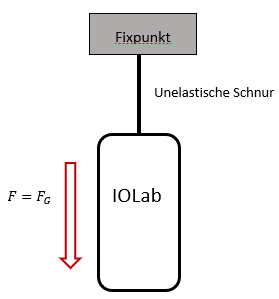
\includegraphics{Massebestimmung}
	\caption[Versuchsaufbau der Massebestimmung]{Schematischer Versuchsaufbau zur Bestimmung der Masse}
	\label{fig:Massenbestimmung}
\end{figure}
\subsection{Bestimmung der Periodendauer}
Nun wird das IOLab an eine Feder statt einer Schnur an dem Kraftsensor und Fixpunkt befestigt und aus dem Ruhepunkt ausgelenkt. Während dessen wird die Kraft $F$ die auf den Kraftsensor wirkt und die Beschleunigung $a$ aufgezeichnet. Man erhält einen Sinus artigen Kraftverlauf aus dem man die Schwingungsperiode auslesen kann. In dem Man die Zeit zwischen fünf Maxima durch vierteilt.
\begin{figure}[H]
	\centering
	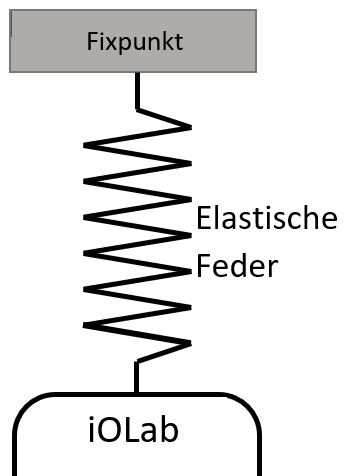
\includegraphics[width=5cm,keepaspectratio]{Schwingung 1}
	\caption[Versuchsaufbau für eine Feder]{Schematische Darstellung des Versuchsaufbau zur Bestimmung der Schwingungsperiode}
	\label{fig:Schwingungsperiode1}
\end{figure}
\subsection{Berechnung der Federkonstante $k$}
Wie in Kapitel \autoref{sec:Grundlagen} diskutiert lässt sich nun der Wert für $k$ durch die Schwingungsperiode und der Masse $m_i$ bestimmen.
\section{Aufstellen eines Modells für parallele Federn}
\label{sec:Modell}
Um ein Modell zur Bestimmung für $k$ aufzustellen wird der Versuch mit der schwersten  Masse $m_3$ mit zwei parallelen Federn wiederholt. Dazu werden mit Hilfe von zwei Kartonstücken parallel aufgehängt. Die Kartonstücke werden mit einer Büroklammer an dem Kraftsensor und dem Fixpunkt befestigt, wie in \autoref{fig:2,3 Federn} zeigt. Anschließend wird da IOLab aus dem Ruhepunkt ausgelenkt und für $20s$ die Kraft $F$ und die Beschleunigung $a$ aufgezeichnet.
\begin{figure}[H]
	\centering
	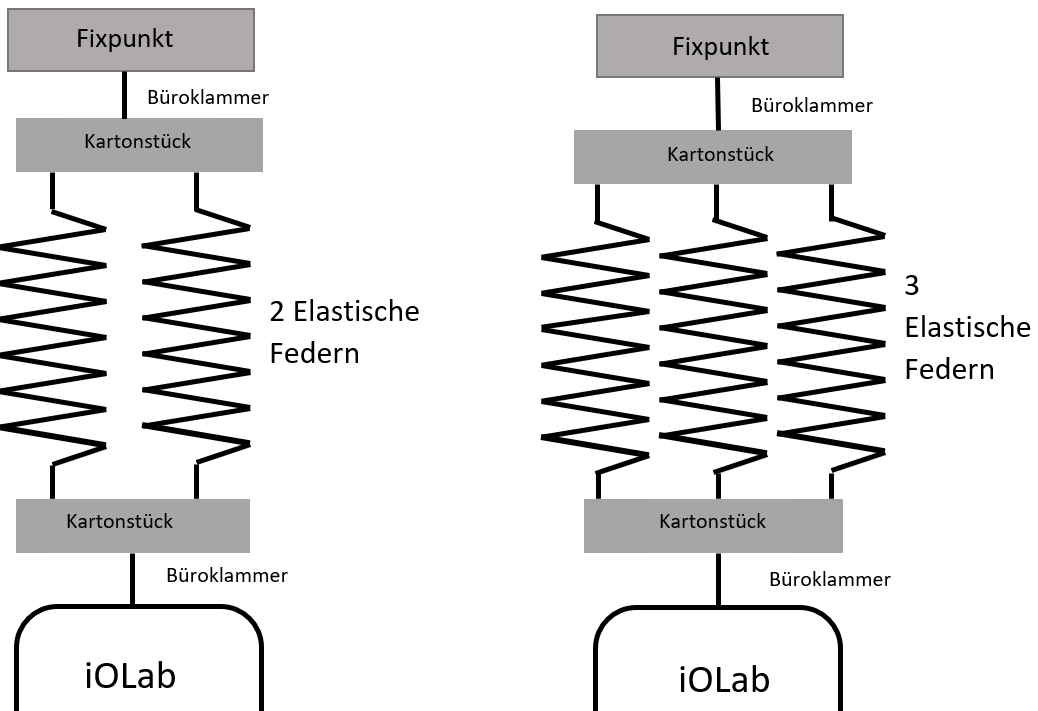
\includegraphics[width=10cm, keepaspectratio]{2,3Federn}
	\caption[Versuchsaufbau mit mehrere Federn]{Schematischer Versuchsaufbau von zwei parallelen Federn(links) und drei Federn (rechts), zur Bestimmung der Periodendauer}
	\label{fig:2,3 Federn}
\end{figure}
Aus dem Vergleich der Federkonstante $k_1$ und der Konstante $k_2$ aus \autoref{sec:Modell} lässt sich nun ein Modell für $N$ federn Aufstellen.
\section{Prüfen des Modell}
Um nun das Modell überprüfen zu können bauen wir ein analoges System mit drei parallelen Federn und der Masse $m_3$, siehe \autoref{fig:2,3 Federn}. Diesmal muss die Auslenkung geringer sein da es sonst zur Überschwingung kommt. Und berechnen $k$ wie in den vorherigen Versuchen.